\documentclass[a4paper,11pt]{article}
%
%--------------------   start of the 'preamble'
%
\usepackage{graphicx,amssymb,amstext,amsmath}
\usepackage{url}
\usepackage{fancybox}
\usepackage[normal]{subfigure}

%
%%    homebrew commands -- to save typing
\newcommand\etc{\textsl{etc}}
\newcommand\eg{\textsl{eg.}\ }
\newcommand\etal{\textsl{et al.}}
\newcommand\Quote[1]{\lq\textsl{#1}\rq}
\newcommand\fr[2]{{\textstyle\frac{#1}{#2}}}
%
%---------------------   end of the 'preamble'
%
\begin{document}
%-----------------------------------------------------------
\title{
  \textbf{\large Temporal and Spatial Databases Project Report}\\
  Multi-dimensional Aggregation for Temporal Data
}

\author{Laura Bledaite}
\maketitle

\section{Introduction}

The objective of this project was to analyze the extension of the multi-dimensional aggregation applied to the data with associated interval values that capture when the data hold. This report describes the Temporal Multi-Dimensional Aggregation (TMDA) operator proposed in~\cite{bohlen} that addresses several challenges posed by interval data. It also reports on an implementation of the operator, on an empirical analysis and compares the results of an empirical study with the ones got in~\cite{bohlen}.

Further the report is structured as follows. In the second section the necessary notation is introduced. In the third section the operator is described and the implementation of two algorithms of the TMDA operator is reported. The fourth section presents the experimental results and their comparison with the results of the previous study. The final section draws the conclusions and suggests future work.

\section{Notation}

It is worth mentioning that all the notation is taken from~\cite{bohlen} and therefore most of the theoretical part is a repetition. The reason of the decision to include it in the report is the necessity of the notation in order to present and discuss the algorithms further on.
 
A discrete \textit{time domain}, $D^{T}$, is assumed here, where the elements are termed time points, following a total order $<^{T}$ . Calendar months with the order $<$ satisfy these requirements, and they are used as a time domain in this report. A timestamp (or time interval) is represented by two chronons, $[T_s, T_e ]$, denoting its inclusive start- and end- points, respectively. $T$ is used as a shorthand for $[T_s, T_e ]$. For timestamps, several relations are introduced: $t \in T$ means that the time point $t$ is included in the interval $T$. For two timestamps $T$ and $T^{'}$, $T^{'} \subseteq T$ iff all time points in $T^{'}$ are also in $T$ , and $T \cap T^{'}$ returns the set of time points in both timestamps. If $T \cap T^{'} \neq \emptyset$, the two intervals are said to overlap.

A \textit{relation schema} is a three-tuple $S = (\Omega, \Delta, dom)$, where $\Omega$ is a non-empty, finite set of attributes, $\Delta$ is a finite set of domains, and $dom: \Omega \rightarrow \Delta$ is a function that associates a domain with each attribute. A temporal relation schema is a relation schema with at least one timestamp valued attribute (the domain of timestamps belongs to $\Delta$). For the purpose of~\cite{bohlen} the temporal relation schemas $R = (A_1, \dots ,A_n,T)$ and $G = (B_1, \dots ,B_m,T)$ were defined and here the definition are borrowed as well. The assumption that relations have a timestamp attribute $T$ was introduced just for convenience. There is no implicit time attribute, and all definitions are parametrized with a timestamp attribute. As usual, the rename operator $\rho$ can be used to adjust schemas as appropriate.

A \textit{tuple over schema} $S = (\Omega, \Delta, dom)$ is a function $r: \Omega \rightarrow \bigcup_{\delta \in \Delta} \delta$, such that for every attribute $A$ of $\Omega$, $r(A) \in dom(A)$. A tuple is temporal iff its schema is temporal. To simplify notation an ordering of attributes is assumed and represented as a tuple $r = (v_1, \dots ,v_n,t)$. A relation over schema $R$ is a finite set of tuples over $R$, denoted as $r$. A couple of shorthands are also used: For a tuple $r$ and an attribute $A$ $r.A$ denotes the value of the attribute $A$ in $r$. For a set of attributes $A_1, \dots , A_m, m < n$, $r[A_1, \dots ,A_m] = (r.A_1, \dots,r.A_m)$.

Three semantics of the association of a non-timestamp attribute with a timestamp attribute are distinguished. For a relation with schema $(A_1, \dots ,A_n,T)$ the attribute characteristics wrt.	$T$ are	given as $CT=	(c_1, \dots , c_n)$, where $c_i \in \{c, m, a\}$. The values $c$, $m$, and $a$ denote constant, malleable, and atomic characteristics, respectively. For example, $CT= (c,m)$ for the schema $(N,H,T)$ means that $N$ has a constant characteristic and $H$ has a malleable characteristic. If several temporal attributes are used, e.g., valid time and transaction time, a non-timestamp attribute can have different characteristics for the two timestamps. In the original paper and also in this report, only one time attribute $T$ is used, and $C$ refers to the characteristics wrt. $T$.

%Definition1. (AdjustmentofAttributeValues)Letr=(v1,...,vn,t)beatupleover schema (A1,...,An,T), I be a timestamp, and let C = (c1,...,cn) be the attribute characteristics. The adjustment of attribute values is defined as follows:
%adj(r,I,C) = (adj(r.A1,r.T,I,c1),...,adj(r.An,r.T,I,cn),I)
% v	i f f c = ’ c ’ adj(v,T,I,c)=v∗|I∩T|/|T| iff c=’m’
%  v	i f f c = ’ a ’ ∧ T = I UNDEF	iff c=’a’∧T ̸=I

Considering the characteristics $C$, the $adj$ function adjusts each non-timestamp attribute value of $r$ to the time interval $I$ and returns the adjusted tuple. For example, for the tuple (Jan , 2000, [2003/01, 2003/12]), the characteristics $(c, m)$, and the time interval [2003/01, 2003/06] the $adj$ function returns (Jan , 1000, [2003/01, 2003/06]).

\section{Implementation of TMDA Operator}

The TMDA operator has two aspects of general temporal aggregation. First one is a case when the timestamp attribute assumes as values the maximal, non-overlapping intervals over which the set of argument tuples is constant. These intervals are called \textit{constant intervals} and they are calculated along with the computation of the aggregate functions while scanning the tuples of the argument relation $r$. The second case is when the result groups with the fixed intervals for which to calculate the aggregate functions are specified in advance and provided as input for the algorithm. These intervals are called \textit{fixed intervals}. 

The implementation of the TMDA operator for constant intervals is based on the following observation: if we scan the argument relation, which is ordered by the interval start values of the tuples, we can at any time point $t$ compute the result tuples that end before $t$ (assuming that no tuples that start after $t$ contribute to these result tuples). Hence, as the argument relation is being scanned, result tuples are produced, and old tuples are removed from main memory. Only the tuples that are valid at time point $t$, termed open tuples, are kept in main memory.

For the use with fixed intervals, the timestamps of the result tuples are specified in the group relation. So, we do not need to maintain the data tuples in main memory, but can process them and update the aggregate values as we scan the data relation.

In the rest of this section two algorithms for the evaluation of TMDA with constant intervals and fixed intervals, respectively, are described, the differences between the implementation suggested in the original paper are pointed.

\subsection{The TMDA-CI Algorithm for Constant Intervals}


  
\subsection{The TMDA-FI Algorithm for Fixed Intervals}





\section{Experiments}

The experiments carried out with the TMDA-CI and TMDA-FI algorithms include the runtime tests for various settings. All experiments were run on an Intel Core 2 Duo personal computer with a 2.4 GHz processor and 2 GB memory.

The data sets used for experiments contain the number of tuples ranging from 200,000 to 1,000,000. As in~\cite{bohlen}, the lifespan of the data relations is $[0,2^{25}]$ and the following types of the data are used for analysis:
\begin{itemize}
\item
$r^{equal}$: All tuples have the same timestamp; $af \in [0.000001, 0.000005]$.
\item
$r^{seq}$: Sequential tuples with one open tuple at each time instant; $af=1$.
\item
$r^{random}$: Start time and duration of the tuples are uniformly distributed in $[0,1200]$ and $[1,1200]$, respectively, with 50153 open tuples on average; $af \in [0.023857, 0.11649]$. In the original paper the random data used was noticeably different. Start time and duration of the tuples were uniformly distributed in $[0,225]$ and $[1,4000]$, respectively, with 33 open tuples on average; $af \in [1.940553, 1.987989]$.
\item
$r^{worst}$: All start and end points are different, and there is a constant interval (in the
middle) where all tuples are open; $af \in [1.999995, 1.999999]$.
\end{itemize}

Here the \textit{aggregation factor} $(af)$ is defined as follows:

Definition 4. (Aggregation factor) The aggregation factor of a temporal aggregation operator is defined as the ratio between the cardinality of the result relation $z$ and the cardinality of the argument relation $r$, i.e., $af = \frac{|z|}{|r|}$.

One more note about the random data set. The distribution is not random from the point of view of the number of open tuples. The randomness is in the start time and duration, therefore the number of open tuples is always small in the beginning and in the end and very high in the middle of the interval. Figure~\ref{open_tuples} shows the distribution of the number of open tuples depending on the time point. 

\begin{figure}[ht!]
\centering 
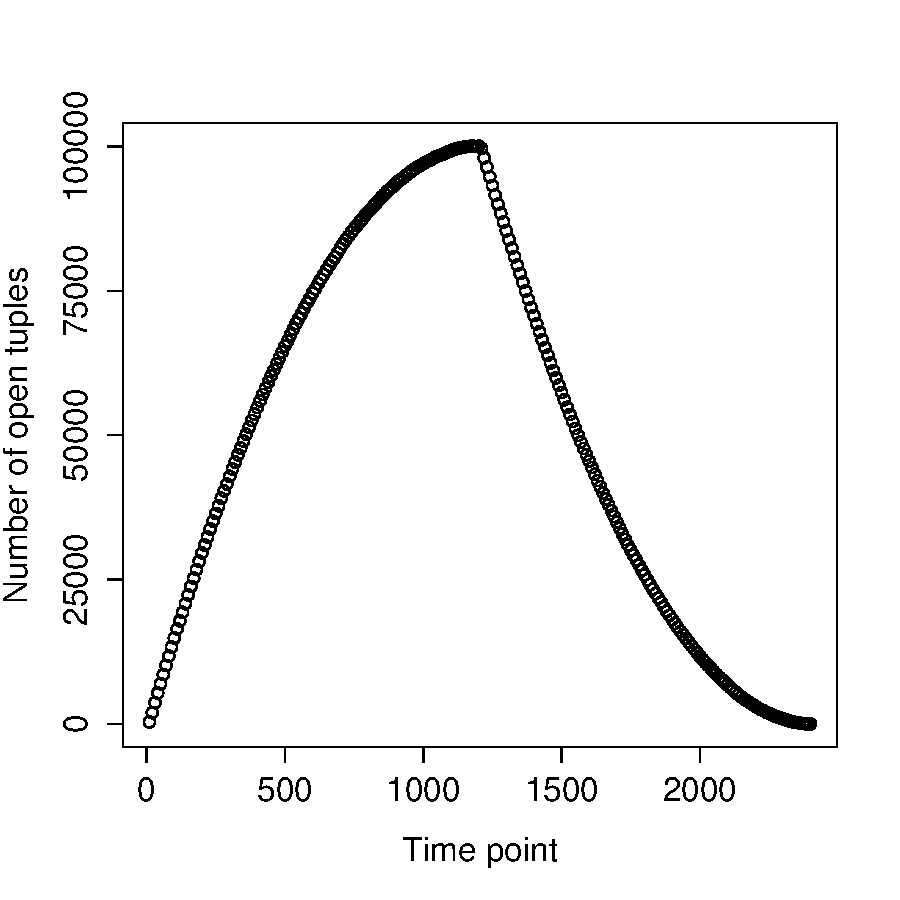
\includegraphics[width=80mm]{../graphs/random_open_tuples.pdf}
\caption{The distribution of the number of open tuples in the random data set.}
\label{open_tuples} 
\end{figure}

\subsection{Scalability of TMDA-CI and TMDA-FI}

The first experiment investigates the scalability of both algorithms: TMDA-CI and TMDA-FI. Figure~\ref{constant_tmda_ci} shows the dependency of the TMDA-CI algorithm on the size of the input relation and the type of the data which is related to the aggregation factor.

The results of the experiment confirm the results of the study carried out by the authors of~\cite{bohlen}. The running times are just negligibly higher than theirs. The difference noticed is in the runtime of the algorithm on $r^{random}$ and the reason is clearly the different data set used.

Relation $r^{worst}$ always has the most open tuples possible and the maximal aggregation factor. For constant intervals it is the only data set from all the used ones that makes the algorithm run in quadratic running time in the size of the input relation. The running time for all the other data sets is linear. Relation $r^{equal}$ with a very small aggregation factor has the smallest running time. Even though the number of open tuples is th ehighest possible, i.e. all tuples from the input relation, they are scanned only once. This makes the algorithm very fast.

For the TMDA-FI algorithm the key parameter that is affecting performance is the number of the result groups stated before the algorthm is started. The performance of TMDA-FI is shown in Figure~\ref{constant_tmda_fi}. In this experiment the results are slightly differet than the authors'. The reason for it is most likely the simper implementation of the algorithm. In our implemetation the index is created using AVL-tree on all the grouping attributes $(B_1,\dots,B_m,T)$. In the experiments only one grouping attribute is used. Therefore, the index is created on $(B,T)$, where $T = [T_s, T_e ]$. Because of the index on multiple attributes, the algorithm becomes noticeably slower. Still, the complexity seems to remain the same.

\begin{figure}[ht!]
	\begin{center}
		\subfigure[constant intervals]{\label{constant_tmda_ci}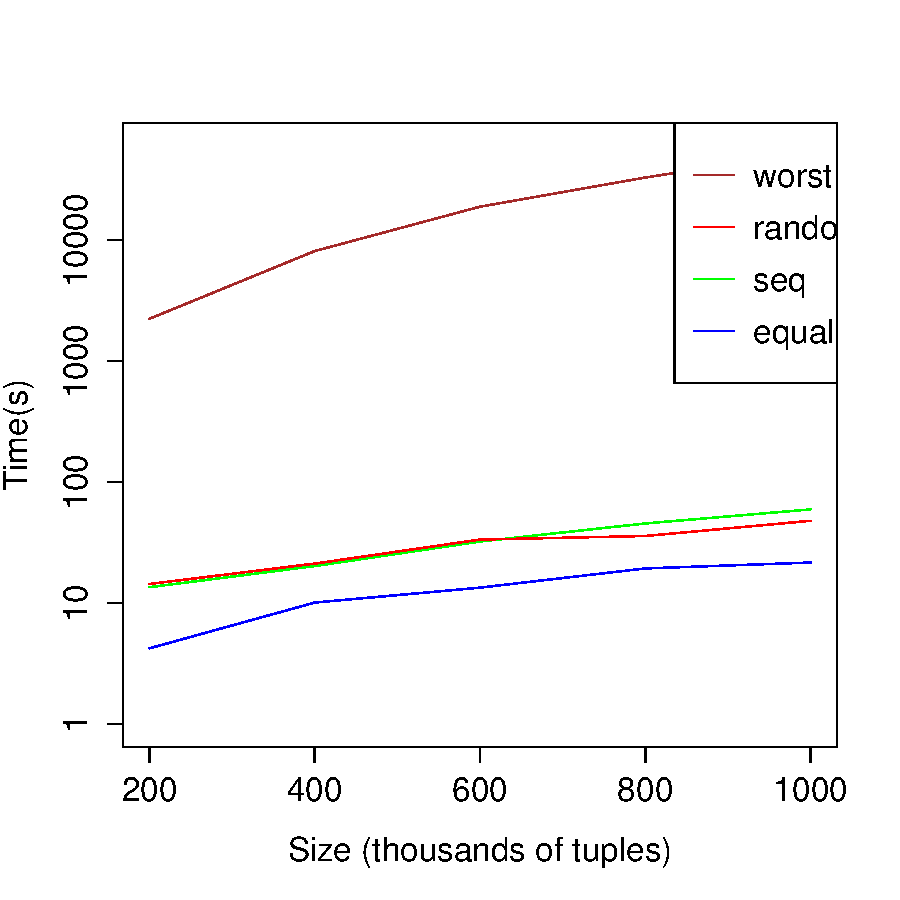
\includegraphics[width=0.4\textwidth]{../graphs/constant_tmda_ci.pdf}}
		\subfigure[fixed intervals]{\label{constant_tmda_fi}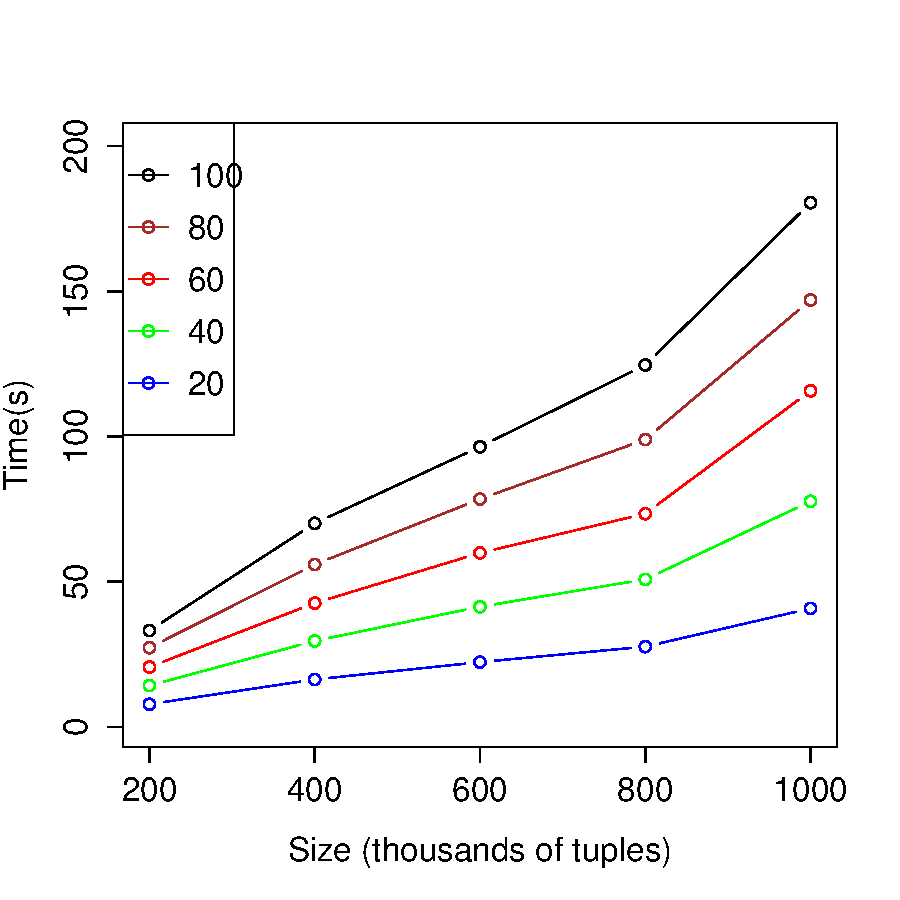
\includegraphics[width=0.4\textwidth]{../graphs/tmda_fi_scalability.pdf}}
	\end{center}
	\caption{Evaluation of TMDA-CI and TMDA-FI.}
	\label{scalability}
\end{figure} 

Figure~\ref{mal_vs_const} show the impact of the attribute characteristics on the performance of the TMDA-CI algorithm. Figure~\ref{mal_vs_const_equal}, Figure~\ref{mal_vs_const_seq} and Figure~\ref{mal_vs_const_random} show the increase of the running time when the result values have to be adjusted for the malable attributes for equal, sequential and random data types respectively. The results suggest that the higher the aggregation factor, the stronger the impact on the runtime of the algorithm, because for each constant interval the algorithm must adjust the result. Thus, the more there are constant intervals, the higher the running time and the impact for the runtime of the same algorithm with the same data just for constant attribute semantics.

\begin{figure}[ht!]
	\begin{center}
		\subfigure[equal]{\label{mal_vs_const_equal}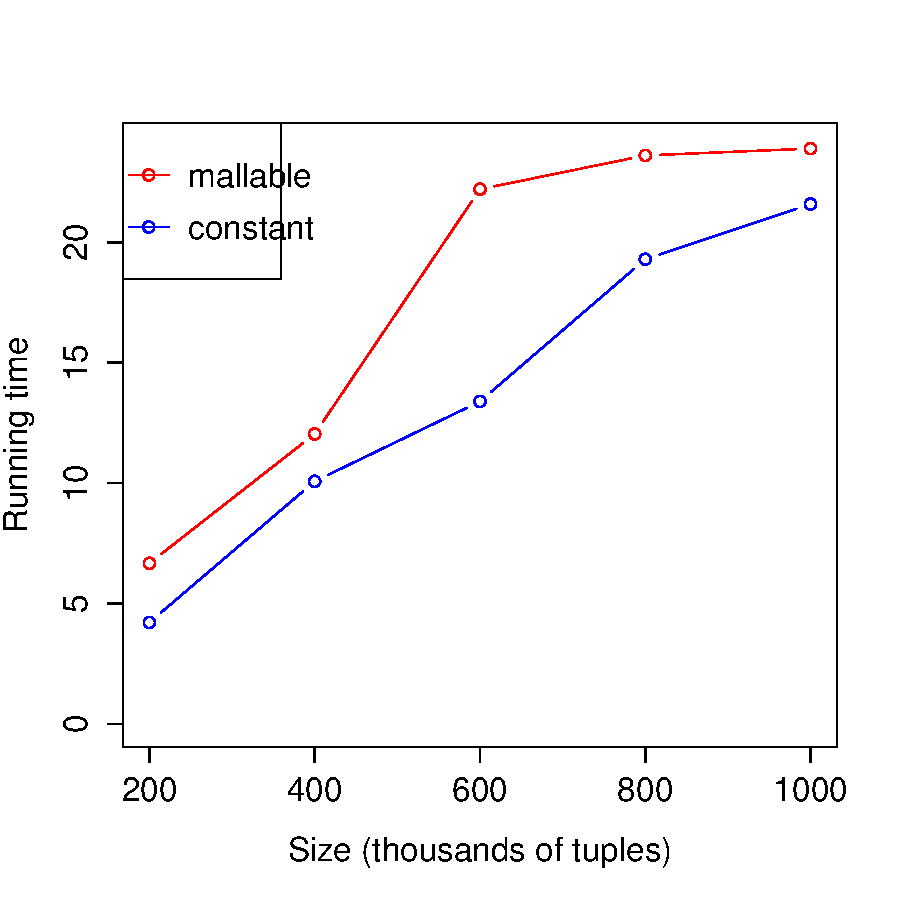
\includegraphics[width=0.3\textwidth]{../graphs/mal_vs_const_equal.pdf}}
		\subfigure[sequential]{\label{mal_vs_const_seq}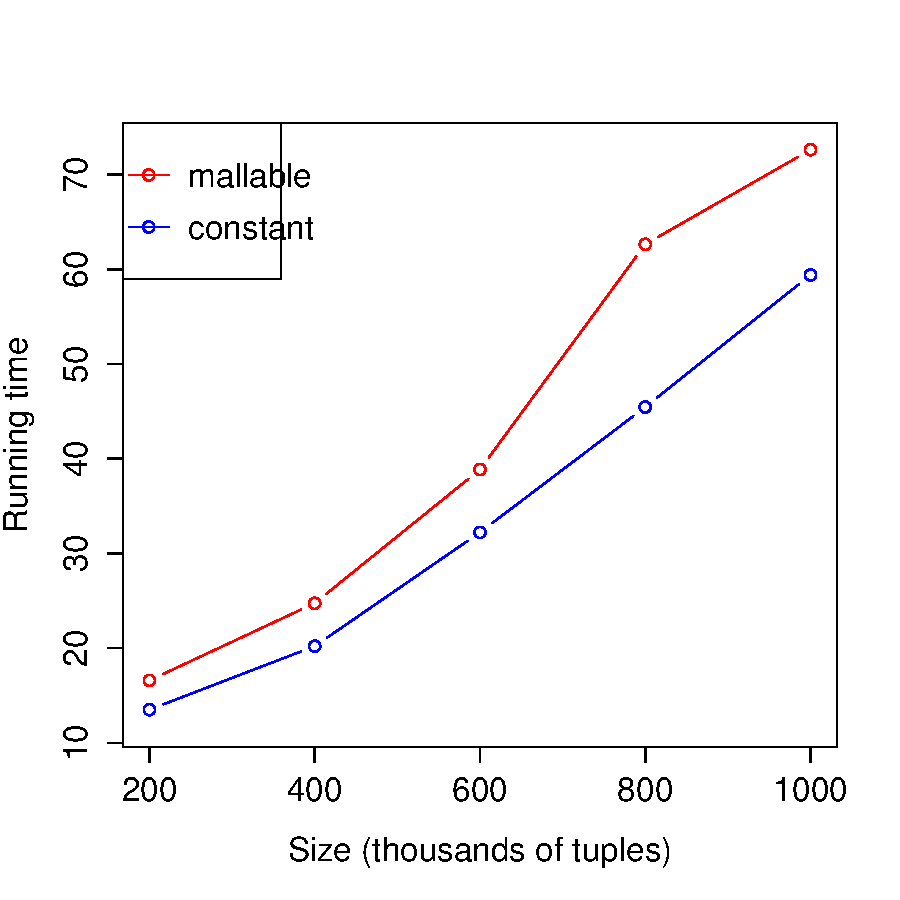
\includegraphics[width=0.3\textwidth]{../graphs/mal_vs_const_seq.pdf}}
		\subfigure[random]{\label{mal_vs_const_random}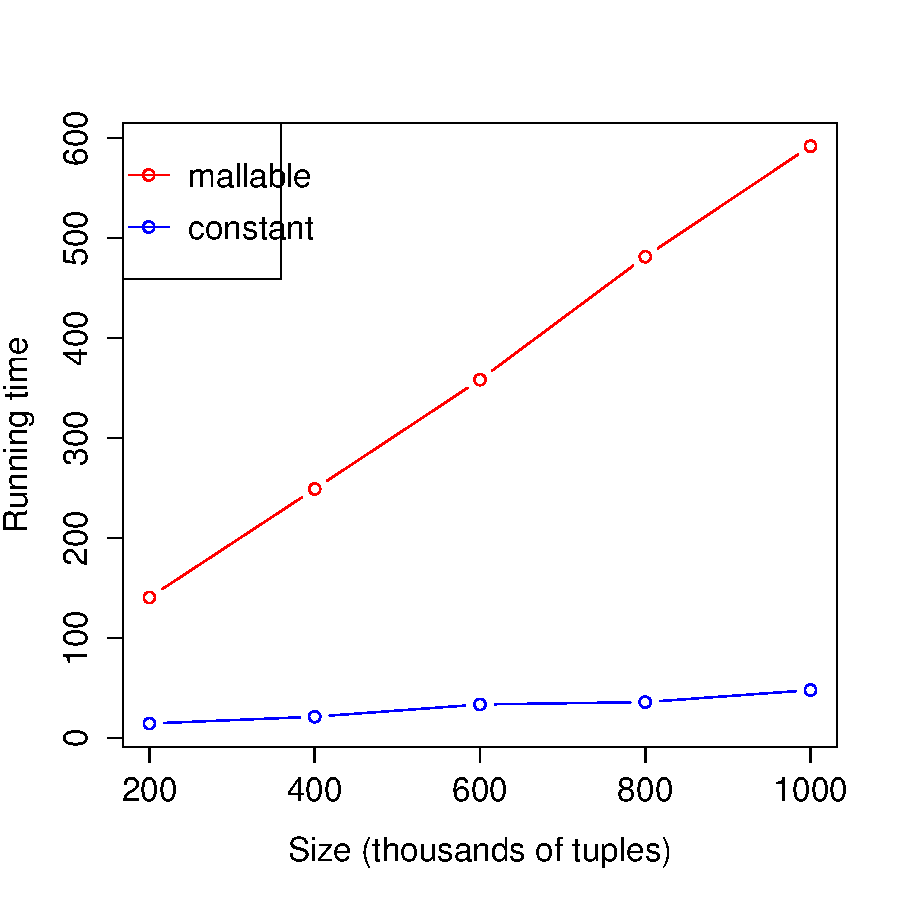
\includegraphics[width=0.3\textwidth]{../graphs/mal_vs_const_random.pdf}}
	\end{center}
	\caption{Comparison of TMDA-CI runtime with mallable and constant attribute characteristics.}
	\label{mal_vs_const}
\end{figure} 

\subsection{Constant Versus Fixed Intervals}

Figure~\ref{sql_tmda_fi} compares the results of two different ways to compute the aggregates with constant interval semantics. One way is simply to run the TMDA-CI algorithm. The other way consists of two steps: (1) precomputation of constant intervals using SQL and (2) running the TMDA-FI algorithm. The results strongly confirm that the TMDA-CI is by far more efficient than the SQL-CI + TMDA-FI. The same results were acquired by the authors. In fact, in our experiment the difference between TMDA-CI and SQL-CI + TMDA-FI is actually much bigger. The reason for that is again the different implementation of TMDA-FI (not sufficiently efficient index) and also the different DBMS used for constant interval precomputation. The authors of the algorithms used Oracle and in this project SQLite3 was used, which as could be expected was much slower.

\begin{figure}[ht!]
\centering 
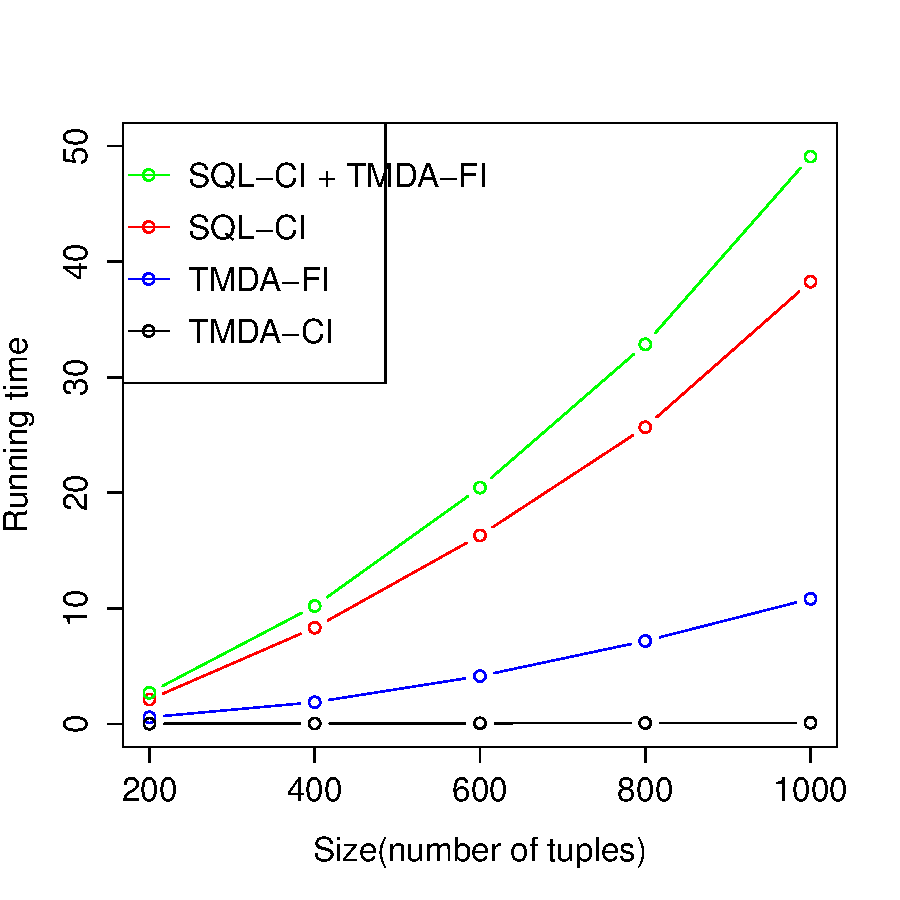
\includegraphics[width=80mm]{../graphs/sql_tmda_fi.pdf}
\caption{Constant vs Fixed Interval Semantics.}
\label{sql_tmda_fi} 
\end{figure}

\section{Conclusions}

The objective of this project was to implement the TMDA-CI and TMDA-FI algorithms  originally presented in~\cite{bohlen}. In this report the implementation of these algorithms was documented, the differences of the implementations were explained and the advantages of the optimizations used in the original implementation were shown. 

Several different experiments were carried out. The results of the experiments that were repeated were compared with the ones acquired in the original study. The differences of the results were explained and the importance of the optimizations was emphasized.

Suggestions for the future work include the search for other optimizations for both algorithms.

%-----------------------------------------------------------
\addcontentsline{toc}{chapter}{\numberline{}Bibliography}

\begin{thebibliography}{9999}
\bibitem{bohlen}
Bohlen M., Gamper J., Jensen C. S.: Multi-Dimensional Aggregation for Temporal Data,
Proceedings of the 10th International Conference on Extending Database Technology: p.p. 257–275, Munich, Germany, 2006.
\end{thebibliography}
\vfill
\begin{flushright}\small Prepared in \LaTeXe\ \end{flushright}

%-----------------------------------------------------------
\appendix
\section{Section Name}
%-----------------------------------------------------------
\end{document}
